\documentclass[10pt,a4paper]{book}
\usepackage[utf8]{inputenc}
\usepackage[spanish]{babel}
\usepackage{mathtools}
\usepackage{amsfonts}
\usepackage{amssymb}
\usepackage{makeidx}
\usepackage{graphicx}
\usepackage{pgf,tikz}
\usetikzlibrary{arrows}
\title{Variable Compleja}
\begin{document}
\chapter{Variable Compleja}%\label{cap.introduccion}
\section{Variable compleja}

Los números complejos se dice $z$ que se puede definir como pares ordenados $$z=\langle x,y\rangle$$ 
de números reales $x$ e $y$ con las operaciones de suma y producto. Se suele identificar los pares $\langle x,0 \rangle$ con los números reales $x$. El conjunto de los números contiene a los números reales como subconjunto. \\
Los números complejos de la forma $\langle 0,y\rangle$ se llama números imaginarios puros. Los números reales $x$ e $y$ en la expresión se conocen respectivamente, como parte real y parte imaginaria de $z$. $$Re\langle z\rangle=x \qquad Im\langle z\rangle=y$$ 
Dos números complejos $\langle x_{1},y_{1} \rangle $ y $\langle x_{2},y_{2} \rangle $ se dicen iguales si tienen iguales la parte real e imaginarios. Es decir $$\langle x_{1},y_{1} \rangle = \langle x_{2},y_{2} \rangle $$ si y solo si $$ x_{1}=x_{2} \wedge y_{1}=y_{2} $$ La suma $ z_{1} + z_{2} $ y el producto $ z_{1} z_{2}$ de dos números complejos $ z_{1}= \langle x_{1},y_{1} \rangle $ y $ z_{2}= \langle x_{2},y_{2} \rangle $ se definen por las ecuaciones $$\langle x_{1},y_{1} \rangle + \langle x_{2},y_{2} \rangle = \langle x_{1} + x_{2}, y_{1} + y_{2} \rangle $$
$$ \langle x_{1},y_{1} \rangle \langle x_{2},y_{2} \rangle = \langle x_{1} x_{2} - y_{1} y_{2}, y_{1} x_{2} - x_{1} y_{2} \rangle $$
En particular $ \langle x, 0 \rangle + \langle 0, y \rangle = \langle x, y \rangle$ y $ \langle 0, y \rangle \langle y, 0 \rangle = \langle 0, y \rangle $ luego $$ \langle x, y \rangle = \langle x, 0 \rangle + \langle 0, 1 \rangle \langle y, 0 \rangle $$
El sistema de los números complejos es un consecuencia una extensión natural de los números reales.\\
Pensando en un número real como $x$ o como $ \langle x,0 \rangle $ y denotamos por $i$ al numero imaginario puro $ \langle 0, 1 \rangle $ podemos ver $$ \langle x, y \rangle = x + y\textit{i} $$
Asimismo con el convenio $ z^{2}= z z, z^{3} = z z^{2} etc...$ Hallamos $$ t^{2} = \langle 0, 1 \rangle \langle 0, 1 \rangle = \langle -1, 0 \rangle $$
Es decir $$ t^{2} = -1 $$ 
Se puede divisar la expresión $$ \langle x_{1} + y_{1}\textit{i} \rangle + \langle x_{2} + y_{2}\textit{i} \rangle = \langle x_{1} + x_{2} \rangle + \langle y_{1} + y_{2}\rangle \textit{i}$$ $$ \langle x_{1} + y_{1}\textit{i} \rangle \langle x_{2} + y_{2}\textit{i} \rangle = \langle x_{1} x_{2} - y_{1} y_{2} \rangle + \langle y_{1} x_{2} + x_{1} y_{2} \rangle \textit{i} $$
Observese que los miembros de la derecha en esas ecuaciones se pueden obtener formalmente manipulando los términos de la izquierda como se sólo contuvieron números numeros reales y sustituyendo como se sólo contuvieron números reales y 
sustituyendo $t^{2} $ por $-1$ cuando aparezca
\definecolor{qqqqff}{rgb}{0,0,1}
\definecolor{xdxdff}{rgb}{0.49,0.49,1}
\definecolor{uququq}{rgb}{0.25,0.25,0.25}
%\label{cap.introduccion}
\section{Conjugacion en C}
\begin{small}
\begin{itemize}
\item 
\emph{DEFINICION.-} Lamaremos conjugado de $z=a+bi$ al número complejo $a-bj$, al cual representaremos por $\overline{z}=a-bi$.
\item
\emph{DEFINICION.-} Dos números complejos son conjugados si diferen solamente en sus partes imaginarias en los signos.
Los números coplejos conjugaso caracterizan puntos simétricos respecto al eje real, así: Si $z=a+bj$ su conjugada es: $\overline{z}=a-bi$\\
\end{itemize}
\end{small}
%\begin{document}
\section{Multiplicación y División en Forma Polar}
Sean $z_1 = r_1(cos\theta_1 + isen\theta_1)$  y  $r_2(cos\theta_2+isen\theta_2)$\\
\\
Dos números complejos en su forma trigonométrica, entonces:\\
$z_1.z_2=r_1(cos\theta_1 +isen\theta_1)r_2(cos\theta_2 +isen\theta_2)=r_1r_2[cos(\theta_1+\theta_2)+isen(\theta_1+\theta_2)]$\\
\\
Si $z_2\neq(0,0)$ y $r_2\neq(0,0)$, entonces:\\
\\
$\displaystyle \frac{z_1}{z_2}=\displaystyle \frac{r_1(cos\theta_1 + isen\theta_1)}{r_2(cos\theta_2 +i sen\theta_2)}=\displaystyle \frac{r_1}{r_2}[cos(\theta_1+\theta_2)+isen(\theta_1+\theta_2)]$\\
\\
Ejemplo:\\
Si $z_1=3(cos\displaystyle \frac{\pi}{6}+isen\displaystyle \frac{\pi}{6})$ y $z_2=4(cos\displaystyle \frac{\pi}{3}+isen\displaystyle \frac{\pi}{3})$\\
\\
Entonces $Z_1.Z_2=(3)(4)[cos(\displaystyle \frac{\pi}{6}+\displaystyle \frac{\pi}{3})+isen(\displaystyle \frac{\pi}{6}+\displaystyle \frac{\pi}{3})]=12(cos\displaystyle \frac{\pi}{2}+isen\displaystyle \frac{\pi}{2})$\\
\\
$\displaystyle \frac{z_1}{z_2}=\displaystyle \frac{4(cos\displaystyle \frac{\pi}{3}+isen\displaystyle \frac{\pi}{3})}{3(cos\displaystyle \frac{\pi}{6}+isen\displaystyle \frac{\pi}{6})}=\displaystyle \frac{4}{3}[cos(\displaystyle \frac{\pi}{3}-\displaystyle \frac{\pi}{6})+isen(\displaystyle \frac{\pi}{3}-\displaystyle \frac{\pi}{6})]=\displaystyle \frac{4}{3}(cos\displaystyle \frac{\pi}{6}+isen\displaystyle \frac{\pi}{6})$
\section{TEOREMA (FORMULA DE MOIVRE)}
\begin{small}
\textbf{Teorema (Formula de MOIVRE)}
Para todo z=a+bi y todo entero positivo n se cumple la siguiente relacion.
$$(a+bi)^{n}=r^{n}(cos n\theta+isen n \theta)$$
Llamada fórmula de MOIVRE
\begin{center}
\textbf{Demostracion}
\end{center}
La demostración lo haremos por inducción
\begin{itemize}
\item Para $n=1, a+bi= r(cos\theta + i sen\theta)$
\item Para $n=h, (a+bi)^{h}=r^{h}(cosh\theta + i senh\theta)$
\item $Para n=h+1,$
$$(a+bi)^{h+1}=(a+bi)^{h}(a+bi)=r^{h}(cosh\theta + i senh\theta)r(cos\theta + i sen\theta)$$
$$(a+bi)^{h+1}=r^{h+1}(cos(h\theta+\theta)+
isen(h\theta+\theta))=r^{h+1}(cos(h+1)\theta+isen(h+1)\theta)$$
Por lo tanto se cumple la formula para todo entero positivo n.
\textbf{TEOREMA.-} Si $z=a+bi$ es un numero complejo y n es un entero positivo. La raiz n - esima de z es:\\
\begin{center}
$z^{\frac{1}{n}}=r^{\frac{1}{n}}[cos \frac{\theta+2kr{n}}{n}+isen\frac{\theta+2kr{n}}{n}]$ para valores de k= 0, 1,......, n.

\textbf{Demostracion}
\end{center}

\end{itemize}
Sea $w=x+iy$, la raiz n - esima de z\\
Es decir: $w^{n}=z$ pero como $z=r(cos\theta+isen\theta)$; $w=p(cos\alpha + isen\alpha)$ $(x+iy)^{n}=a+bi$, reemplazando se tiene: $p^{n}(cos n\alpha+i sen n\alpha)=r(cos\theta + isen\theta)$ de donde $p^{n}=r$, $\alpha n=\theta+2k\Pi$, k= 0, 1, 2, ....., n-1\\
Luego $p=r^{\frac{1}{n}}$, $\alpha=\frac{\theta+2k\Pi}{n}$, k= 0, 1, 2,....,n-1\\
Como $w=p(cos \alpha + i sen \alpha)$ se tiene: $w=r^{\frac{1}{n}}[cos \frac{\theta+2k\Pi}{n}+i sen\frac{\theta+2k\Pi}{n}]$ como $w$ es la raiz n - esima de $z$, se tiene:
\begin{center}
$Z^{\frac{1}{n}}=^{\frac{1}{n}}[cos\frac{\theta+2k\Pi}{n}+isen\frac{\theta+2k\Pi}{n}]$ para k=0, 1, 2,...., n-1
\end{center}
\textbf{TEOREMA.-} Sea $z=a+ai$, definimos $z^{\dfrac{m}{n}=(z^{\frac{1}{n}}})^{m}$, para m y n enteros positivos donde $m$ y $n$ son primos entre si, se cumple la relacion siguiente:
$$z^{\frac{m}{n}}=r^{\frac{m}{n}}[cos\frac{m}{n}(\theta+2k\Pi)+isen\frac{m}{n}(\theta+2k\Pi)]$$
siendo $r=\sqrt{a^{2}+b^{2}}$, $\theta=arctg(\frac{b}{a})$

\end{small}
\section{Logaritmo en C} 
La exponencial compleja $z=re^{i\theta}$ es un número complejo, el valor de $\theta$ se denomina argumento principal de $z$, que denominaremos por: $\theta=\arctan(z)$\\\\
Para todo complejo $z\neq0$, le corresponde solamente un valor de $\theta$ con $0\leq\theta\leq2\pi$\\
Sin embargo cualquier otro intervalo de longitud $2\pi$ por ejemplo $-\pi\leq\theta\leq\theta$ se puede emplear\\\\
El logaritmo complemento es la inversa de la exponencial compleja, es decir:\\
Si $z=re^{i\theta}$ es un número complejo $\Rightarrow \exists w \in C$ único tal que $r=\Vert z \Vert$ y $\theta=\arctan(z)$\\\\
Generalizando se tiene que:
\begin{center}
\fcolorbox{red}{white}{ \color{black} $\ln z=w=\ln r +i(\theta +2k\pi)$}\\
\end{center}
El valor pincipal de $\ln z$es el que se obtiene cuando $k=0$, es decir:\\
V.P. de $\ln z=\ln r+i\theta$\\\\
{\bf Ejemplo}\\\\
Hallar $\ln z$, donde $z=1-i$\\\\
\begin{center}
\bf Desarrollo
\end{center}
$z=1-i \Rightarrow r=\Vert z \Vert=\sqrt{2}$\\\\
$\tan\theta=\frac{-1}{1} \Rightarrow \theta=\frac{7\pi}{4}$\\\\
$\ln z=\ln(1-i)$\\\\
$\ln r+i(\theta+2k\pi)$\\\\
$\ln \sqrt{2}+i(\frac{7\pi}{4}+2k\pi)$\\\\
$\ln \sqrt{2}+(\frac{7}{4}+2k)\pi i$\\\\
y el Valor Principal(V.P.)de\\\\
$\ln Z=\ln\sqrt{2}+\frac{7\pi}{4}i$
\section{EXPONENCIAL COMPLEJA GENERAL}
Sea $z_1$ y $z_2$ donde $z_1 \neq 0$, entonces consideramos una exponencia compleja $w = z_1^{z_2}$ aplicando el logaritmo de base natural tenemos:
 \\ $ln w = ln z_1^{z_2} = z_2 ln z_1$
 \\ por definición tenemos que: \begin{equation}
 w = e^{z_2 ln z_1}
\end{equation}  
%Funciones Complejas
 \textbf{FUNCIONES COMPLEJAS DE VARIABLE COMPLEJA}
 \\ a) \textbf{Definición.-} Una función de variable compleja $y$ de valor compleja es una regla que asigna un número complejo $w$ a cada número complejo $z$ del conjunto $S$, es decir: $f:$ $S\subset C \rightarrow C$
 \begin{center}
	\begin{equation}
	z \rightarrow f(z)=w
    \end{equation}	   
   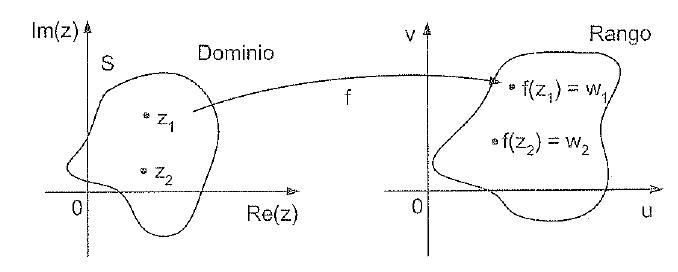
\includegraphics[scale=0.8]{Funcion.png}  
  \end{center}  
 Si $w =f(z)$ es el valor de la función $f$ en el punto $z$ que están en el dominio $S$. 
 \\ A la función $w=f(z)$ expresaremos en términos de la descomposición en parte real e imaginaria es decir:
 \\ Si $z= x + jy$ y $w = u +jv$ entonces $w =f(z)=f(x+jy)=f(x,y)=u(x,y)+jv(x,y)$ , por lo tanto la función compleja $w=f(z)$ de una variable compleja esta formado por un par de funciones reales de dos variable resales, es decir:
  \begin{equation}
   w = f(z) = u(x,y) + jv(x,y) 
  \end{equation}
  donde $u(x,y) = Re(f(z))$ , $v(x,y)=Im(f(z))$ , además $u,v: R^{2} \rightarrow R $ son funciones reales de dos variables
  \\
  \textbf{Observación}
  \begin{enumerate}
   \item Al Conjunto de números complejos que puede tomar la función $w=f(z)$ conforme "z" varia en la región S, se llama      Rango de Valores de la función $w=f(z)$
   \item Si $\forall z \in S$ le corresponde solamente un valor $w=f(z)$ , entonces la función se llama "UNÍVOCA" (uno a uno) \\ \begin{center}
    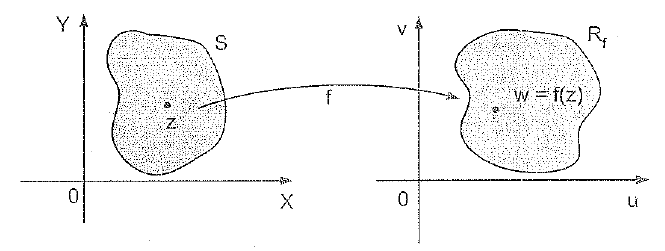
\includegraphics[scale=0.6]{univoca.png}
   \end{center}
   En caso contrario se llama "multiforme"
   \item La función $w=f(z)$ realiza una transformación de los puntos del plano complejo (z) en los puntos correspondientes al plan complejo (w)
  \end{enumerate}     
%Propiedades de Límites de Funciones
\textbf{PROPIEDADES DE LÍMITES DE FUNCIONES COMPLEJAS} \\
Supongamos que $ \lim_{z\to\ z_0} f(z)=A$ y $ \lim_{z\to\ z_0} g(z)=B$ , entonces: \\
\begin{enumerate}
 \item $ \lim_{z\to\ z_0} (f(z) + g(z))=\lim_{z\to\ z_0} f(z) + \lim_{z\to\ z_0} g(z) = A + B$
 \item $ \lim_{z\to\ z_0} (f(z) - g(z))=\lim_{z\to\ z_0} f(z) - \lim_{z\to\ z_0} g(z) = A - B$
 \item $ \lim_{z\to\ z_0} (f(z).g(z))=\lim_{z\to\ z_0} f(z) . \lim_{z\to\ z_0} g(z) = A.B$
 \item Si $ \lim_{z\to\ z_0} f(z) = A \neq 0$ , probar que existe $\delta > 0$ , tal que $||f(z)|| > \dfrac{1}{2} ||A||$ para $||0<||z-z_0||<\delta$
 \item Si $ \lim_{z\to\ z_0} f(z) = A \neq 0$ , entonces $ \lim_{z\to\ z_0} \dfrac{1}{f(z)} = \dfrac{1}{A}$
 \item $ \lim_{z\to\ z_0} \dfrac{f(z)}{g(z)}) = \dfrac{lim_{z\to\ z_0} f(z)}{lim_{z\to\ z_0} g(z)} = \dfrac{A}{B}$ , $B\neq 0$ , $g(z) \neq 0$ , $\forall z$
 \item Si $f(z) = a_{n} z^{n} + a_{n-1} z^{n-1} + ... + a_{1} z + a_{0}$, una función polinómica $z$, entonces: 
 $\lim_{z\to\ z_0} f(z) =lim_{z\to\ z_0} (a_{n} z^{n} + a_{n-1} z^{n-1} + ... + a_{1} z + a_{0})$
 \begin{center}
  $=a_{n} z_{0}^{n} + a_{n-1} z_{0}^{n-1} + ... + a_{1} z_0 + a_{0}$
 \end{center}
 \item Si $lim_{z\to\ z_0} f(z) = L_1$ y $lim_{z\to\ z_0} g(z) = L_2$ entonces $L_1=L_2$ (propiedad unicidad)
 \item Si $lim_{z\to\ z_0} f(z) = A$ y $lim_{z\to\ A} g(z)$ existen: si $\exists V_\rho (z_0)$ tal que $f(z) \neq z_0$ , $\forall z \subset V_\rho (z_0)$ entonces $lim_{z\to\ z_0} g(f(z)) = lim_{z\to\ A}  g(z)$ 
  
\end{enumerate}

\end{document}
